% use "amsart" instead of "article" for AMSLaTeX format
\documentclass[a4paper,11.5pt]{report}   
\renewcommand{\baselinestretch}{1.5} 

\usepackage[strings]{underscore}
\usepackage{datetime}

\newdateformat{monthyeardate}{%
  \monthname[\THEMONTH], \THEYEAR}

\usepackage{enumerate}

\usepackage{setspace}

%\usepackage[margin=1.2in]{geometry}

\usepackage[a4paper,bindingoffset=0.4in,%
            left=1in,right=1in,top=1in,bottom=1in,%
            footskip=.25in]{geometry}
            


% ... or a4paper or a5paper or
\geometry{a4paper}      
             		
% Activate to begin paragraphs with an empty line rather than an indent
\usepackage[parfill]{parskip}   

 % Use pdf, png, jpg, or eps§ with pdflatex; use eps in DVI mode		
\usepackage{graphicx, wrapfig}				

\setcounter{secnumdepth}{4}

\usepackage{nomencl}
\makenomenclature

\usepackage{lipsum}

\usepackage{gensymb}

%\usepackage[monochrome]{color}
%\usepackage[utf8]{inputenc}


\usepackage{float}

\usepackage{amsmath}
	\numberwithin{figure}{section}
	\numberwithin{table}{section}
	\numberwithin{equation}{section}

\usepackage{amsmath}
	\numberwithin{equation}{section}
	\newcommand*{\Scale}[2][4]{\scalebox{#1}{$#2$}}%
	
\usepackage{multirow}

\usepackage{appendix}

\usepackage{array}

%\newcolumntype{P}[1]{>{\centering\arraybackslash}p{#1}}

\usepackage{blindtext}

\usepackage[export]{adjustbox}[2011/08/13]
	
\usepackage{gensymb}
	
\usepackage{colortbl}

\usepackage{longtable}

\usepackage{tabularx}

\usepackage{enumerate}

\newcommand{\gray}{\rowcolor[gray]{.90}}

\makeatletter
\newcommand*{\rom}[1]{\expandafter\@slowromancap\romannumeral #1@}
\makeatother

\usepackage{rotating}

%\bibliographystyle{unsrtnat}
\usepackage{natbib}
\newcommand*{\urlprefix}{Available from: }
\newcommand*{\urldateprefix}{Accessed }
\bibliographystyle{bathx}
%\usepackage[sort&compress,numbers]{natbib}


\usepackage[final]{pdfpages}

\usepackage{caption}

\usepackage[% line break after label
   singlelinecheck=off, font=bf]{caption}
%\newcommand{\rom}[1]{%
%  \textup{\expandafter{\romannumeral#1}}%
%}

\usepackage{tocloft}
\renewcommand{\cftpartleader}{\cftdotfill{\cftdotsep}} % for parts
\renewcommand{\cftchapleader}{\cftdotfill{\cftdotsep}} % for chapters
 \renewcommand\cftchapafterpnum{\vskip10pt}

 
%\usepackage{titletoc}% http://ctan.org/pkg/titletoc
%\titlecontents*{chapter}% <section-type>
%  [0pt]% <left>
%  {}% <above-code>
%  {\bfseries\chaptername\ \thecontentslabel.\quad}% <numbered-entry-format>
%  {}% <numberless-entry-format>
%  {\bfseries\hfill\contentspage}% <filler-page-format>


\usepackage{subfig}					%use figure packagesx

\makeatletter

\newcommand\frontmatter{%
    \cleardoublepage
  %\@mainmatterfalse
  \pagenumbering{Roman}}

\newcommand\mainmatter{%
    \cleardoublepage
 % \@mainmattertrue
  \pagenumbering{arabic}}

\newcommand\backmatter{%
  \if@openright
    \cleardoublepage
  \else
    \clearpage
  \fi
 % \@mainmatterfalse
   }

\makeatother

\usepackage{fancyhdr}
\fancyhf{}
  \fancyhf[lef,rof]{\thepage}%
\pagestyle{fancy}
\fancypagestyle{plain}{%
  \fancyhf{}%
  \renewcommand{\headrulewidth}{0pt}%
  \fancyhf[rof]{\thepage}%
}

\usepackage{memhfixc}

\renewcommand{\contentsname}{Table of Contents}

\usepackage{pdflscape}

\usepackage{lscape}

\usepackage{textcomp}

%\usepackage[libertine,cmintegrals,cmbraces,vvarbb]{newtxmath}

%\usepackage[sorting=none]{biblatex}

\usepackage{notoccite}

\usepackage{titlesec}
\usepackage{appendix, apptools}
\AtAppendix{%
\titleformat{\chapter}[display]{\vspace*{-30pt}\bfseries\huge}{\chaptername~\thechapter}{1em}{}
\titlespacing*{\chapter}{0pt}{0pt}{0pt}}%

\makeatletter
\newcommand{\mypm}{\mathbin{\mathpalette\@mypm\relax}}
\newcommand{\@mypm}[2]{\ooalign{%
  \raisebox{.1\height}{$#1+$}\cr
  \smash{\raisebox{-.6\height}{$#1-$}}\cr}}
\makeatother

\usepackage{afterpage}
\newcommand\blankpage{%
    \null
    \thispagestyle{empty}%
    \addtocounter{page}{-1}%
    \newpage}
    
\usepackage{url}

\usepackage[official]{eurosym}

\usepackage{enumitem}


%\title{
%Development an Educational Game to Teach SQL Programming
%}
%\author{
%Amarnath Kakkar \\
%\normalsize University of Bath
%}
%\date{}							% Activate to display a given date or no date


\begin{document}

\frontmatter


%titlepage
\clearpage\thispagestyle{empty}
\begin{center}
\begin{minipage}{0.9\linewidth}
    \centering
%University logo
    \vspace{0.8cm}
    
\includegraphics[width=0.4\linewidth]{logobath.jpg}\par
    
    \vspace{2.5cm}
%Thesis title
    \vspace{0.2cm}
    {\uppercase{\Large \textbf{Development of an Educational Game to Teach Conditional and Iterative Control Structures} \par}}
    \vspace{3cm}
%Author's name
    {\Large \textbf{Amarnath Kakkar}\par}
        \vspace{3cm}
% $^{\circ}$
    {\large A final year project submitted in partial fulfilment for the degree of Bachelor's in Computer Science and Mathematics with Honours\par}
    {\large University of Bath\par}
    \vspace{4.5cm}
%supervisor and date
    {\large \textbf{\monthyeardate\today}\par}
    \vspace{1cm}
\end{minipage}
\end{center}

\afterpage{\blankpage}




\clearpage\thispagestyle{empty}
\begin{center}
\begin{minipage}{0.9\linewidth}
%University logo

\vspace{10cm}
{This dissertation may be made available for consultation within the University Library and may be photocopied or lent to other libraries for the purposes of consultation.\par}
\vspace{1cm}
Signed: 
   	
	
\end{minipage}
\end{center}

\newpage



    
\clearpage\thispagestyle{empty}
\begin{center}
\begin{minipage}{1\linewidth}
%Thesis title
%    \vspace{0.2cm}
%    {\uppercase{\large {Submitted in partial fulfilment for the degree of masters in aerospace engineering} \par}}
    \vspace{2cm}
%%Author's name
    {\LARGE Development of an Educational Game to Teach Conditional and Iterative Control Structures \par}
    \vspace{1cm}	
    {\large Submitted by: Amarnath Kakkar\par}
	
    \vspace{1.5cm}
    {\Large \textbf{COPYRIGHT}\par}
    \vspace{0.5cm}
    {Attention is drawn to the fact that copyright of this dissertation rests with its author. The Intellectual Property Rights of the products produced as part of the project belong to the author unless otherwise specified below, in accordance with the University of Bath?s policy on intellectual property
(see http://www.bath.ac.uk/ordinances/22.pdf).
This copy of the dissertation has been supplied on condition that anyone who consults it is understood to recognise that its copyright rests with its author and that no quotation from the dissertation and no information derived from it may be published without the prior written consent of the author.\par}

     \vspace{0.5cm}
     {\Large \textbf{Declaration}\par}
      \vspace{0.5cm}
      {This dissertation is submitted to the University of Bath in accordance with the requirements of the degree of Bachelor of Science in the Department of Computer Science. No portion of the work in this dissertation has been submitted in sup- port of an application for any other degree or qualification of this or any other university or institution of learning. Except where specifically acknowledged, it is the work of the author.\par}
    
     \vspace{2.5cm}
%% $^{\circ}$
    {\large Department of Computer Science\par}
    {\large University of Bath\par}
    \vspace{0.5cm}
%supervisor and date
    {\large Supervisor: Dr. Alan Hayes}\par
    {\large \textbf{\monthyeardate\today}\par}
    \vspace{1cm}
\end{minipage}
\end{center}

\afterpage{\blankpage}

\hfill

\section*{\Huge{Abstract}}

To be written.



\newpage

\addtocontents{toc}{\protect\setstretch{1}}
\tableofcontents

\newpage
{%
\let\oldnumberline\numberline%
\renewcommand{\numberline}{\figurename~\oldnumberline}%
\listoffigures%
}

\newpage
\listoftables  

\newpage
\hfill

\section*{\Huge{Outline of Project}}

To be written.

\newpage
\hfill
\section*{\Huge{Acknowldgements}}

To be written.
 
\afterpage{\blankpage}

\mainmatter

\chapter{Introduction}

%use Breuer2010 to define game
%Platform: Personal Computer
%Subject Matter: Programming fundamentals - Conditional and iterative Control Structures
%Learning Goals: Programming skills
%Learning Principles: Trial and Error
%Target Audience: First year university students
%Interaction Mode: Single Player
%Application Area: Academic Learning
%Controls/Interfaces: Mouse & Keyboard
%Common Gaming Tags: 2D Maze Adventure


\afterpage{\blankpage}

\chapter{Literature Review}
%\section{Aims of This Section}

%This Literature Review aims to bring together various studies, and provide an insight into the use of games for educational purposes. It also aims to critically evaluate the material for any consistencies or inconsistencies, and to hopefully provide another perspective on the field.

%\subsection{Defining Serious Games}
%In the area of gamification, various definitions of serious games are found. Most commonly, and perhaps quite broadly, the term 'serious game', is defined as, digital games used for purposes other than mere entertainment \cite{Susi2416}.  While a variety of definitions have been suggested, this dissertation will use the definition suggested by \cite{Garris2002} who saw it as "instructional games that are designed for training or to promote learning" together with "games that do not have entertainment, enjoyment or fun as their primary purpose"  \cite{MichaelChen2006}. However, it is not to say that serious games should not be entertaining, enjoyable or fun.

%\subsection{Outline of Review}
%This review will; identify the benefits of serious games, and make clear any negatives, go through examples of serious games and their approaches, including any specific game design elements implemented, and outline any techniques that seem to be of positive influence or negative influence, look into existing resources for teaching SQL and outline the trade-offs with each approach, finally bring together these ideas summarise various points.

%\section{Benefits of Serious Games}
%Today's students are brought up in the digital era. \cite{Prensky2001} refers to them as 'Digital Natives', that have experienced a new form of video game play, which brings opportunities with great potential for their learning. Thus potentially making games great learning environments within education. However, \cite{Girard2013} summarises that there is need for more empirical research to determine the effectiveness of serious games. On the other hand, \cite{Pieter2013} reports that in general, serious games are more effective than traditional teaching methods, and that more studies are required to determine the effects of various features.

%In this section, we will outline some of the empirical researches that exist on the internet.

%\subsection{}

%\section{Examples of Serious Games}
%\subsection{Game Design Elements}
%\section{Existing Methods for Teaching SQL}
%\section{Summary}


\section{Video Games}

%The academic study of games, ludology, is a relatively new and emerging field. As the video game revolution took off in the late 20th century, so did academic interest in games. 

%Video games for entertainment have dominated the market, 

%The academic study of games, is a relatively new and emerging field. Games are naturally creative things, however academics see the potential in games for a variety of different reasons, and so game design frameworks have been developed to help design and create games.

The video games industry has grown very rapidly in recent years, and is expected to continue to grow. The current market value is predicted as \$150 billion USD and is predicted to reach \$180 billion by 2022 \citep{vgamesResearch}. In 2006, video games were considered as one of the most popular forms of entertainment in the United States \citep{sherry2006, ritterfeld2006}. Currently, video games are considered a popular form of entertainment globally.

%At one time, particu- larly in the 1970s, the term video games meant ?games played in a video arcade.?

\citeauthor{Botturi2009} claimed that video games in the 1970s meant "games that were playeable in amusement arcades" \citep{Botturi2009}. Since then, a video game can be defined as "a mental contest, played with a computer according to certain rules for amusement, recreation, or winning a stake" \citep{Zyda2005}.

%Military applications have dominated the market, but civil applications are expected to grow [8][9]. UAV have already proved to be successful in field operations however, further research can enable UAV?s to be used in intelligence gathering, such as stealth and combat operations [34].

%\subsection{History}

%The earliest documented predecessor to video games was observed in 1948, when the "Cathode-Ray Tube Amusement Device" was patented. The amusement device, required players to overlay pictures of targets such as airplanes in front of the screen \citep{Thefirstvideogame}.

%Ten years later, physicist William A. Higinbotham was credited for creating the first video game. Displaying his research at an exhibition, he anticipated that his demonstration would not generate any interest, so he conceptualised and created 'Tennis for Two' \citep{TennisForTwo}. Tennis for Two was created using an analog computer with an oscilloscope for a screen. It was the first game to display motion and allow multiple players to play together \citep{Thefirstvideogame}. 

%The rise of modern generation of video games is credited to the development of 'Spacewar!' in 1962, 'Computer Space' in 1971 and 'Pong' in 1972. Spacewar! was developed for academic purposes to test the limits of new hardware, but shortly after became quite popular. Spacewar! was played by Nolan Bushnell, who used the idea of the game to create Computer Space, although, Computer Space did not gain much popular traction. This was partly due to its long winded instructions and complex game controls. Learning from these mistakes, the creators of Computer Space decided to create a simpler game and came up with the idea for Pong, which became very popular. Computer Space and Pong were designed solely for entertainment, and Pongs popularity was credited to the simplicity of its design \citep{Lowood2009}.

%In the late 1980s, video games became a mainstream media industry \citep{Dmitri2003}.

\subsection{Impacts}


Initially, the majority of research on the effects of playing video games focused on the negative impacts, such as the potential aggression, addiction and depression from 'gaming'. However, researchers have argued that a more balanced perspective is needed \citep{Granic2014}. Playing video games has been linked to an increase in perceptual, cognitive, behavioural, affective and motivational abilities \citep{Connolly2012}. Studies have also demonstrated that there are positive impacts from playing violent games, such as increased visuospatial skills \citep{Ferguson2007}. 

\subsection{Uses}

Video games are now used for a wide variety of reasons. They are becoming increasingly useful in the global education and training market. Apart from entertainment, video games are being used in: military, government, education, corporate and healthcare \citep{Johann2015}.

%Many attempts to pinpoint the creation of the very first video game have been made. However, the creation of the first modern video game is commonly dated to 1958. first video game ever invented was developed by a physicist William Higinbotham, in 1958. The game was called 'Tennis for Two'. The design and concept was conjured up from an instructional book the inventor was reading at the time \cite{TennisForTwo}.

%The first recorded video game invented, was developed by a physicist called William Higinbotham, called 'Tennis for Two' in 1958. The concept of the game, came from an instructional book that he was reading at that time \cite{TennisForTwo}.

%In 1970, R. Barton discusses the evolution of 'The Imaginit Management Game' and the development of a game model. This model consisted of a set of rules, such that a management game could be repurposed to fit another management scenario \cite{Barton1970}.

%First a set of generality aspirations were defined, and then a set of strategies 'describes features of "generalized" management computer game and then reports a case history of adapting this game model, which was designed for ideal generality, to an application that challenged that very generality.

%\section{Benefits of Video Games}

%\subsection{Platforms}

\section{Educational Games}

The term 'Serious Game' can be used to describe an educational game. A serious game refers to a game that has an educational purpose and is not intended to be played primarily for entertainment \citep{abt1970}. 

Serious games became an established academic field of study in 2007, after establishment of The Serious Games Institute \citep{Wilkinson2016}. The market value of the serious games industry in 2016 was predicted at \$1.5 billion USD, and is predicted to reach \$9 billion in 2023 \citep{alliedmarketresearch}.

\subsection{Definition}

There is currently no singleton definition for term 'Serious Game'. \citeauthor{Johann2015} argue that, groups and individuals define the term depending on their perspectives and interests, and that there are a wide variety of groups and individuals focusing on different issues \citep{Johann2015}. The first recorded definition of the term was set out in 1970 by \citeauthor{abt1970} \citep{Wilkinson2016}, who defined it as follows: "Games that have an explicit and carefully thought-out educational purpose, and are not intended to be played primarily for amusement. This does not mean that serious games are not, or should not be, entertaining." \citep{abt1970}. In \citeyear{Michael2005}, \citeauthor{Michael2005} built on this definition to come up with the definition that they are "Games that do not have entertainment, enjoyment or fun as their primary objective" \citep{Michael2005}. This definition suggested that serious games are not limited to only educational purposes. The commonly agreed upon definition closely matches the definition by \citeauthor{Michael2005} \citep[see][]{Johann2015}.

Another definition that is often referred to was set out by Zyda \citep[see][]{Johann2015}. This definition however contradicts the one set out by \citeauthor{Michael2005} \citep{Johann2015}. In contrast, \citeauthor{Michael2005} argue that serious games should not, have entertainment or fun as their primary objective. On the other hand, \citeauthor{Zyda2005} expressed that the entertainment component of the game should come first, and also that the story of the game is more important than the pedagogy \citep{Zyda2005}. His definition is as follows: "a mental contest, played with a computer in accordance with specific rules, that uses entertainment to further government or corporate training, education, health, public policy, and strategic communication objectives" \citep{Zyda2005}. However this definition also suggests that serious games can only be digital \citep{Jean}. 

Since there are a variety of definitions, for this dissertation, I will use the one provided by \citeauthor{abt1970} and work entertainment around the primary purpose of the game - to teach.

%"Educational game" is still a newly emerging thing in our country, and there is no explicit definition nowadays. Narrowly speaking, educational game refers to the integration of education and game, and the education effect naturally generated from the process of playing games, in other words, it means "a type of computer game software which generates education effect through interest" \cite{song2008}



%There is a difficulty defining the term ?serious game?, as there appears to be a contradiction between its constituents terms; ?serious? and ?game? seem to be mutually exclusive \cite{Johann2015}. 


%The first constituent, ?serious?, is according to Ben Sawyer (in Michael and Chen, 2006) intended to reflect the purpose of the game, why it was created, and has no bearing on the content of the game itself. Regarding the second constituent, already Wittgenstein (1953) showed that there are difficulties in defining the concept of a game. There simply are no necessary and sufficient conditions \cite{Johann2015}.


%\subsubsection*{Instructional Games} %get rid of these when finished

%An instructional game is defined as "a type of software function designed to increase motivation by adding game-like rules and/or competition to a learning activity" \cite{Roblyer2013}.

%However, \citeauthor{AtsusiHirumi2010}, define an instructional game as "an interactive, digital game (e.g., adventure, strategy, role-play, action, and massive multiplayer online games) that is designed specifically to facilitate learning" \cite{AtsusiHirumi2010}.

%\citeauthor{Hays2005} defined instructional games , instruction must be designed to support specific instructional objectives, which are determined by job requirements. Second, instruction must include the opportunity for a learner to interact with the instructional content in a meaningful way. Third, the student's performance must be assessed to determine if he or she has learned what was intended. Finally, the results of the assessment must be presented to the student in a relevant and timely manner to either reinforce correct actions or to provide remediation for incorrect actions.

%\subsubsection*{Serious Games} %get rid of these when finished

%There are many definitions for the term 'Serious Game', but most agree on a core meaning that serious games are (digital) games used for purposes other than mere entertainment. \citeauthor{Zyda2005}, defined them as "a mental contest, played with a computer in accordance with specific rules, that uses entertainment to further government or corporate training, education, health, public policy, and strategic communication objectives" \cite{Zyda2005}.
%So for the purpose of this dissertation, we will focus on the subset of serious games that are concerned with educational purposes.

%Video games for entertainment purposes have dominated the market, however serious games are expected to grow. Serious games have proved to be successful, however further research is required to determine the effectiveness of such games \cite{Susi2416}.

%This dissertation aims to create a game for learning in educational contexts. Thus this game fits all the above definitions.

\subsection{History}

Educational games have arguably existed since the 7th century. Among the oldest is the board game 'Chaturgana', which is argued by historians to be the precursor to chess \citep{Wilkinson2016}. The aim of the game was to teach officers to become better planners for battles \citep{Wilkinson2016}. Another board game created more recently - in the 20th century was 'Landlord's Game'; a precursor to monopoly. It was designed to illustrate the dangers of capitalist approaches to land taxes and property renting \citep{Wilkinson2016}. So we can see that, games designed to educate, have existed for a long time.


%The interest in UAV?s has been observed since 1916, when the first modern unmanned aircraft was invented, Hewitt?s UAV. This was a result of Sperry?s work, on the flight stabilisation using gyroscope devices, which provided flight stabilisation [11]. This attracted the interest of the US Navy however, due to technical difficulties the research and work in automatic planes was lost. In 1933 the Royal Navy Queen bee?s target drone was operated for the first time and the potential of UAV?s was understood, but it still required perfection of remote operations. Reginald Denny then developed the successful target drone RP-2, during WWII using radio control [12].

%During the Cold war, the development in reconnaissance missions increased and the first recon- naissance UAV was developed, called the MQM-57 Falconer [13]. Not long after, the Ryan Model 147 was launched, which was the first unmanned aircraft which is known as an UAV today. In conclusion, the importance and usefulness of UAV was demonstrated over the years and is now being further researched, focusing on longer endurance UAV?s and MAV?s [12].

%Interest in flying wing designs for both UAV?s and larger scale civil applications, are now being revisited.

The interest in digital educational games, has been observed since 1967, when the first educational program was developed, 'Logo Programming' \citep{hayes2008} . Logo programming was an environment that allowed players to utilise the programming language LOGO in order to learn mathematics \citep{feurzeig1969}. Logo was popular among schools in the US \citep{lehrer1986}, and it became a key part of educational strategies research \citep{hayes2008}. 

Academic interest in games that could be used for purposes apart from entertainment emerged emerged in \citeyear{abt1970} by \citeauthor{abt1970}, in his book \textit{Serious Games} \citep{Breuer2010}. The rise in digital games around this time created an opportunity for developing serious games \citep{Wilkinson2016}. 

However, serious games did not gain much traction until 2002, when a game developed by the US Army, became hugely popular. 'America's Army' was developed as a training and recruitment game for the military. It is now considered as the forefront of modern serious games \citep{Zyda2005, Wilkinson2016}. In conclusion the potential of using games as educational tools has been demonstrated for a long time, and is now being further researched and developed, focusing on training and education in a number of different industries \citep{Wilkinson2016}.

%In 1971, 'The Oregon Trail' was released. The Oregon Trail was created by history teachers, to cover American history in 1848 \citep{Jean}. This game became hugely popular, and now has several sequels and spinoffs. The rise in arcade games and home consoles around this time, created an opportunity for developing serious games \citep{Wilkinson2016}.

 
%Learning in games appears indisputable considering recent studies, but when it comes to the question of what and how players learn through playing games, controversial answers can be found \citep{Mitgutsch}.

%Around this same time, the power and potential of computer games for education and training was beginning to be uncovered \citep{neil2005}. Computer games were hypothesised to provide multiple benefits, such as: 

%\begin{itemize}
%\item Complex and diverse approaches to learning processes and outcomes
%\item Interactivity
%\item Ability to address cognitive as well as affective learning issues
%\item Motivation for learning
%\end{itemize}

%America's Army
%\subsection{Benefits}


%Computer games are defined as games that are played on Personal Computers, and video games as games played using a television and a games console \citep{Cummings07}.

%In 1958, Tennis for Two was created using an analog computer and oscilloscope for a screen. Four years later, Spacewar was developed using a digital minicomputer and a cathode-ray tube as the display, making it one of the first computer games. In 1972, Computer space and Pong were among the first video games. They were played on televisions placed in upright cabinets, and this paved the look and feel for future arcade games \citep{TennisForTwo, Lowood2009}.

%Computer games separated from video games in the early 1990s. Since then, 3D home consoles like the Sony Playstation and the Sega Saturn have been introduced. Some innovations to consoles include; touchscreen and motion control \citep{Cummings07}. Recently, we have seen the development and the use of Virtual Reality consoles for gaming, entertainment and learning \citep{vrhaptics}.

\subsection{Benefits}

Serious games have become an interesting area for multidisciplinary academic research \citep{Breuer2010}. There are interests from fields such as psychology, computer science, pedagogy, sociology and cultural studies \citep{Breuer2010}. Many studies have looked into and discussed the benefits of serious games in educational contexts, and I will discuss some of these below.

\subsubsection{E-learning}

E-learning can be defined as an approach to teaching and learning, based on the use of electronic media and devices \citep{sangra2012}. Thus, digital educational games can be seen as a type of e-learning.

Educational games have inherent beneficial properties. For instance, they are able to provide information on demand and just in time, and in the context of actual use and people's purposes and goals, something that does not often happen in schools \citep{Gee2003}.

Other properties of e-learning include: ease of accessibility; can be used in absence of teachers or instructors; provide opportunities for relations between learners, helping eliminate the potential of hindering participation; low cost per person served; allows self-pacing - allowing student to study at their own pace; high level of interactivity; ability to use attractive graphics, and is an engaging and entertaining activity \citep{arkorful2015, Girard2013}.

In a study carried out on what university students thought about e-learning, students reported that they expected e-learning to be an integral part of the learning process within higher education \citep{Connolly2012}. Thus, the use of a digital game in higher education, may not be an unfounded concept to students.

%Games are able to provide information on demand and just in time, not out of the contexts of actual use or apart from people's purposes and goals, something that happens too often in schools. People are quite poor at understanding and remembering information they have received out of context or too long before they can make use of it \cite{Gee2003}. 

%Games allow players to be producers and not just consumers. Along with the designer, the player's actions co-create the game world \cite{Gee2003}.

\subsubsection{Learning Through Games}


Games can be a great learning environment \citep[see][]{prensky2003, Gee2003}. Despite the vast research on the negative impacts of gaming, playing video games identified for imparting beneficial skills such as, visual attention, spatial skills, problem solving skills and creativity \citep{Granic2014}. 

When players first begin a new game, they first learn the rules and the controls of the game, then use this newly acquired knowledge to complete objectives or levels. As players progress through the game, it becomes more difficult and calls for them to use better skills and knowledge for them to move to the next stages of the game. \citeauthor{vygotsky1978} coined the term \textit{the zone of proximal development}, where students gain a higher degree of learning when they are presented with tasks which are just beyond their current level of ability but may require some help to complete \citep{vygotsky1978}.

Today's learners have grown up immersed in digital technology \citep{Prensky2001}; \citeauthor{Prensky2001} calls this generation of people 'Digitial Natives', because they have spent long periods of time playing video games \citep{prensky2003}. In 2016, 2.5 billion people were reported to actively play video games worldwide \citep{Statista}, and a year later, roughly 57\% were aged between 10 and 35 \citep{Statistanewzoo}. Therefore, this generation will be more receptive to computer-based learning \citep{Girard2013}.

Playing games is naturally a fun and pleasurable activity \citep{Prensky2001}, and research has shown that fun is important for the learning process, as learners can be more motivated and willing to learn \citep{Bisson1996, Cordova1996}. Learners' enjoyment of a game has also been shown to improve learners' acquisition of knowledge \citep{giannakos2013}.

%Games which also provide an optimal balance of challenge and frustration, leave players in a motivated state to continue to play \citep{Gee2003}.

%This motivational ?sweet spot? balances optimal levels of challenge and frustration with sufficient experiences of success and accomplishment

\subsubsection{Effectiveness of Learning through Games}

Evidence of learning through educational games has been demonstrated \citep{Connolly2012, Pieter2013, Girard2013}. However, the effectiveness of educational games is undetermined \citep{Connolly2012, Girard2013}. There are also different viewpoints when it comes to determining their effectiveness. Two such meta-analyses, \citet{Pieter2013} and \citet{Girard2013}, explored at the effectiveness of learning through games, and made different conclusions. These studies are compared in Table \ref{tab:effectivess learning comparison}.

\begin{table}[H]
\centering
\caption{Comparison of meta-analyses on the effectiveness of learning through games}
\label{tab:effectivess learning comparison}
\begin{tabular}{p{3.4cm} | p{5cm} | p{5cm}}
       & \textbf{\citet{Pieter2013}}                  & \textbf{\citet{Girard2013}}               \\ \hline
\textbf{Types of Games}  & Serious games                & Serious games \& video games               
\\ \hline
\textbf{Measuring}   & Learning, retention and motivation                   & Learning and engagement              
\\ \hline
\textbf{Learning Outcomes}	& Knowledge or skill acquisition 	& Knowledge or skill acquisition
\\ \hline
\textbf{Instructional Domain}	& Biology, maths, language or engineering	& Various (including: academic knowledge, cognitive skills, professional knowledge, cancer therapies)
\\ \hline
\textbf{Studies Published Between}		& 1990 - 2012		& 2007 - 2011
\\ \hline
\textbf{Experimental Design of Studies}		& Posttest or pretest-posttest		& Atleast pretest-posttest
\\ \hline
\textbf{Studies Reviewed} & 39                         & 9		                 
\\ \hline
\textbf{Age Range of Studied Population} & Wide range                         & 9 - 47		                 
\\ \hline
\textbf{Results support effective learning through games} & Yes                         & Inconclusive
\end{tabular}
\end{table}


\citeauthor{Pieter2013} found that serious games were more effective in terms of learning and retention when compared to conventional teaching methods, but not more motivating. On the other hand, \citeauthor{Girard2013} found that only a few of the games resulted in improved learning, with the others having no difference when compared to traditional methods of teaching. A point to note is that in \citet{Pieter2013}, serious games were compared to lectures, reading, drill and practice, or hypertext learning environments, whilst in \citet{Girard2013}, they were compared to face-to-face lessons, pencil-and-paper studying or no studying at all. The former is a more modern way of teaching, whereas the latter is very limited.

\citeauthor{Pieter2013} evaluated a broad spectrum of studies, whereas \citeauthor{Girard2013} only evaluated randomised control trial studies. \citeauthor{Pieter2013} argued that if they only considered the studies with randomised samples with a pretest-posttest design, similar to \citeauthor{Girard2013} study, the positive effects in favour of serious games may disappear. 

In conclusion, there is a need for more empirical research to determine the effectiveness of serious games, and this is being addressed \citep{Connolly2012}.


%\citeauthor{Girard2013} evaluated 6 serious games, and of these 6, \citeauthor{Pieter2013} evaluated 3 of them.


%\citeauthor{Pieter2013} compared serious games to more modern instructional methods, such as lectures, reading, drill and practice, or hypertext learning environments, whilst \citeauthor{Girard2013} compared them to more traditional methods, such as face-to-face lessons or pencil-and-paper studying.

%\citeauthor{Pieter2013} found that serious games were more effective in terms of learning and retention, but they were not more motivating than conventional instruction methods. This study also measured the effectiveness of using serious games in conjunction with other instructional methods, and this was found to be the most effective means of learning \citep{Pieter2013}.

%Whilst \citeauthor{Girard2013} found that only a few of the games resulted in improved learning, with the others having no difference when compared to traditional methods of teaching. The study concluded that it was impossible to draw any conclusions on the effectiveness of serious games.



%\citep[see][]{Pieter2013, Girard2013}


%However, despite  in a meta-analysis on the effectiveness of serious despite the potential of using games in educational environments, studies do not  \citep{Mitgutsch, Connolly2012}.

%In a meta-analysis on the effectiveness of learning and engagement of games for learning, \citeauthor{Girard2013} covered six serious games and five video games. Finding that 2 out of the 6 supported having a positive impact on learning compared to other types of training or no training, 1 showed no difference and 3 had no beneficial effect on learning \citep{Girard2013}. This study however looked at a small number of serious games. They also could not draw a conclusion about the effectiveness of serious games, arguing that there is a wide variety of types and uses for serious games.

%Analyses show that games promote learning. Games can support the development of a number of different skills; analytical and spatial skills, strategic skills and insight, learning and recollection capabilities, psychomotor skills, visual selective attention.


%ELSPA, 2006; Gee, 2005, 2007; Klopfer et al., 2009; Robertson, 2009; Shaffer, 2007

%Kirkpatrick?s four levels for evaluating training

%Baker and Mayer?s CRESST model of learning

%\subsubsection{Engagement}

%Prensky, 2001

%Good games operate at the outer and growing edge of a player's competence, remaining challenging, but do-able, which is a very motivating state for human beings \citep{Gee2003}.

%In a meta-analysis conducted by \citeauthor{Connolly2012} on the positive impacts of games, they found that students reported enjoying game-based approaches to learning and that they find them motivating \citep{Connolly2012}.

%\subsubsection{Feedback}

%\citeauthor{Gee2008} argued that people learn best from their experiences when they get immediate feedback during those experiences so that they can recognise and assess their errors and see where their expectations have failed \citep{Gee2008}. As an example, Cameron and Dwyer (2005) (as cited in \cite{Connolly2012}) found that including feedback into educational game about the accuracy of users answers, lead to improved performance in terms of knowledge acquisition.


\subsection{Examples}

There are many existing educational games designed to teach various topics. I will cover some educational games and interesting technologies that help further programming skills.

\subsubsection*{Scratch}

Scratch is a block-based visual programming language and an online community for sharing, discussing and 'remixing' one another's projects. Projects can range from creating your own interactive stories, games, animations or simulations, which users can share with one another online \citep{resnick2009}. Today, Scratch has accumulated almost 40 million users, with the core audience between ages 8 and 16, which have created and shared more than 40 million projects \citep{scratchstats}.

The Scratch language is based on a collection of programming blocks that can be snapped together to create programs. Scratch blocks are shaped in a way such that they can only fit with other blocks  to make syntactic sense (see Figure \ref{fig:Scratch-Example}). The creator of Scratch and fellow researchers argued that the social aspect of Scratch was important for it to succeed, with a user claiming that she learnt a lot about different kinds of programming by looking at, downloading, and modifying the scripts from other peoples games. Users can also work together on projects, helping them develop their collaborative and team leadership skills \citep{resnick2009}.

%The ages of Scratch users extend beyond 16; up until 80 \citep{scratchstats}, and 


%, with the aim of improving first-time programmers' experiences. 
Scratch has also been used in higher educational contexts \citep{resnick2009}. In a study conducted by \citet{malan2007}, Scratch was used at Harvard's summer school to introduce students to programming. After a total of five hours on Scratch, students transitioned onto Java for the remainder of the course. \citeauthor{malan2007} found that more than 75\% of students felt that using Scratch, was a positive influence with their transition onto Java; a more complex syntactical language \citep{malan2007}. It is clear from the student responses that Scratch helped develop their computational thinking skills. This is often hard to do in languages like Java as students can feel overwhelmed trying to learn the complex syntax, which can hinder their ability to learn to program \citep{Koulouri2014}.

%More than 75\% of the students reported that Scratch was a positive influence, with some reporting that it was fun and easy to use. From the responses presented in the study, it is clear that Scratch helped students improve their computational thinking skills, which seemed to have greatly helped when transitioning into Java. 

%This suggests that removing the burden of having to learn the syntax, of more so complex syntactical languages like Java \citep{malan2007}, in introductory courses, can help motivate students to learn programming.


\begin{figure}[H]
 \centering
    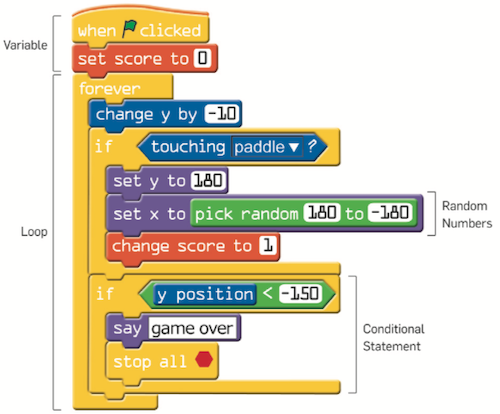
\includegraphics[width=0.7\textwidth]{Scratch-Example}
       \captionsetup{justification=centering}
\caption{An example of a Scratch script  {\citep{resnick2009}}}
\label{fig:Scratch-Example}
\end{figure}

\subsubsection*{Prog\&Play}

Prog\&Play was developed to tackle the issue of student motivation in computer science courses in higher education. Prog\&Play is a 3D real-time strategy game designed to strengthen programming skills. It was built on top of an existing open-source multiplayer game, because of the potential advantage of the game already being robust. The developers of Prog\&Play created an API that enabled students to interact with the game through programmable commands, as the original game did not contain any programming \citep{muratet2011}.

Prog\&Play introduced variables, functions and conditional and iterative control structures. The game is based on a war between the factions, 'Systems', 'Hackers' and 'Networks' (see Figure \ref{fig:ProgAndPlay-Example}). Players choose a side and give orders to their units through a set of commands. The developers also created a single player mode, where students could be gradually introduced to learning topics and learn how to play. The multiplayer aspect then allowed students to create their own programs and compete with each other \citep{muratet2011}.

Through examinations conducted by the teachers, \citeauthor{muratet2011} found that students who played the game achieved better marks than those who did not. Many students who played the game went on to choose a computer science unit the next semester, compared to those that did not play the game at all. Interestingly, a majority of students preferred the programming version, Prog\&Play, to the original game which did not require any programming \citep{muratet2011}.

\begin{figure}[H]
 \centering
    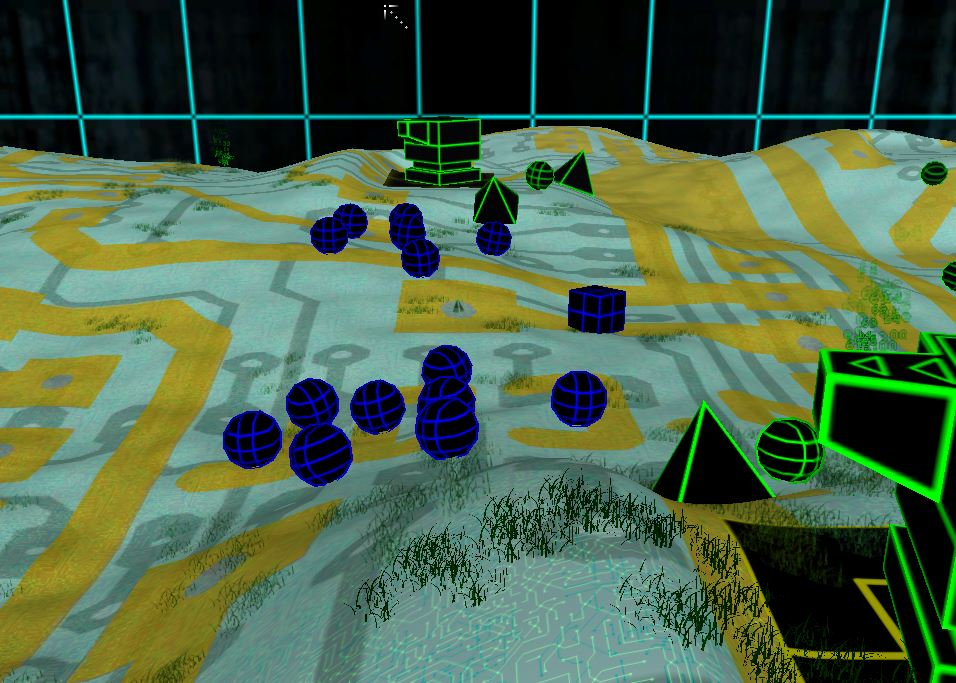
\includegraphics[width=0.7\textwidth]{ProgAndPlay-Example}
       \captionsetup{justification=centering}
\caption{A screenshot of the game Prog\&Play {\citep{progplaywebsite}}}
\label{fig:ProgAndPlay-Example}
\end{figure}


\subsubsection*{Gidget}

Gidget is a web-based game developed as part of a study to improve learning in novice programmers. The study tested the effects of personifying programming tool feedback. One such personification was to programming errors that were displayed to users \citep{lee2011}. 

In the case of Gidget, you have have to work with a damaged robot, also named Gidget, to help clean up a city and protect its animals after a chemical spill. The robot, Gidget, acts as a companion and feedback tool. It uses personified language, takes the blame for syntax and runtime errors, and has an emotional face \citep{lee2011}. \citeauthor{lee2011} claimed that this would change the role of the conventional feedback tool often perceived as an authoritative figure, which can be off-putting, to a collaborator needing assistance. The game teaches the design and analysis of basic algorithms in a language designed specifically for the game. Players have to debug the code produced by Gidget to complete the levels \citep{lee2011}.

\citeauthor{lee2011} carried out a study with 116 participants, using two versions of the game. One version was with a personified Gidget robot (see Figure \ref{fig:Gidget-Example}), and the other with a Gidget that had a faceless screen that provided impersonal feedback. The results revealed that the group using the personified Gidget, completed more levels in roughly the same amount of time in comparison to the group using the faceless Gidget, suggesting that the personification of feedback had a positive effect on participations' motivation to play. Although, the personification of Gidget did not affect the enjoyment felt playing the game \citep{lee2011}.


\begin{figure}[H]
 \centering
    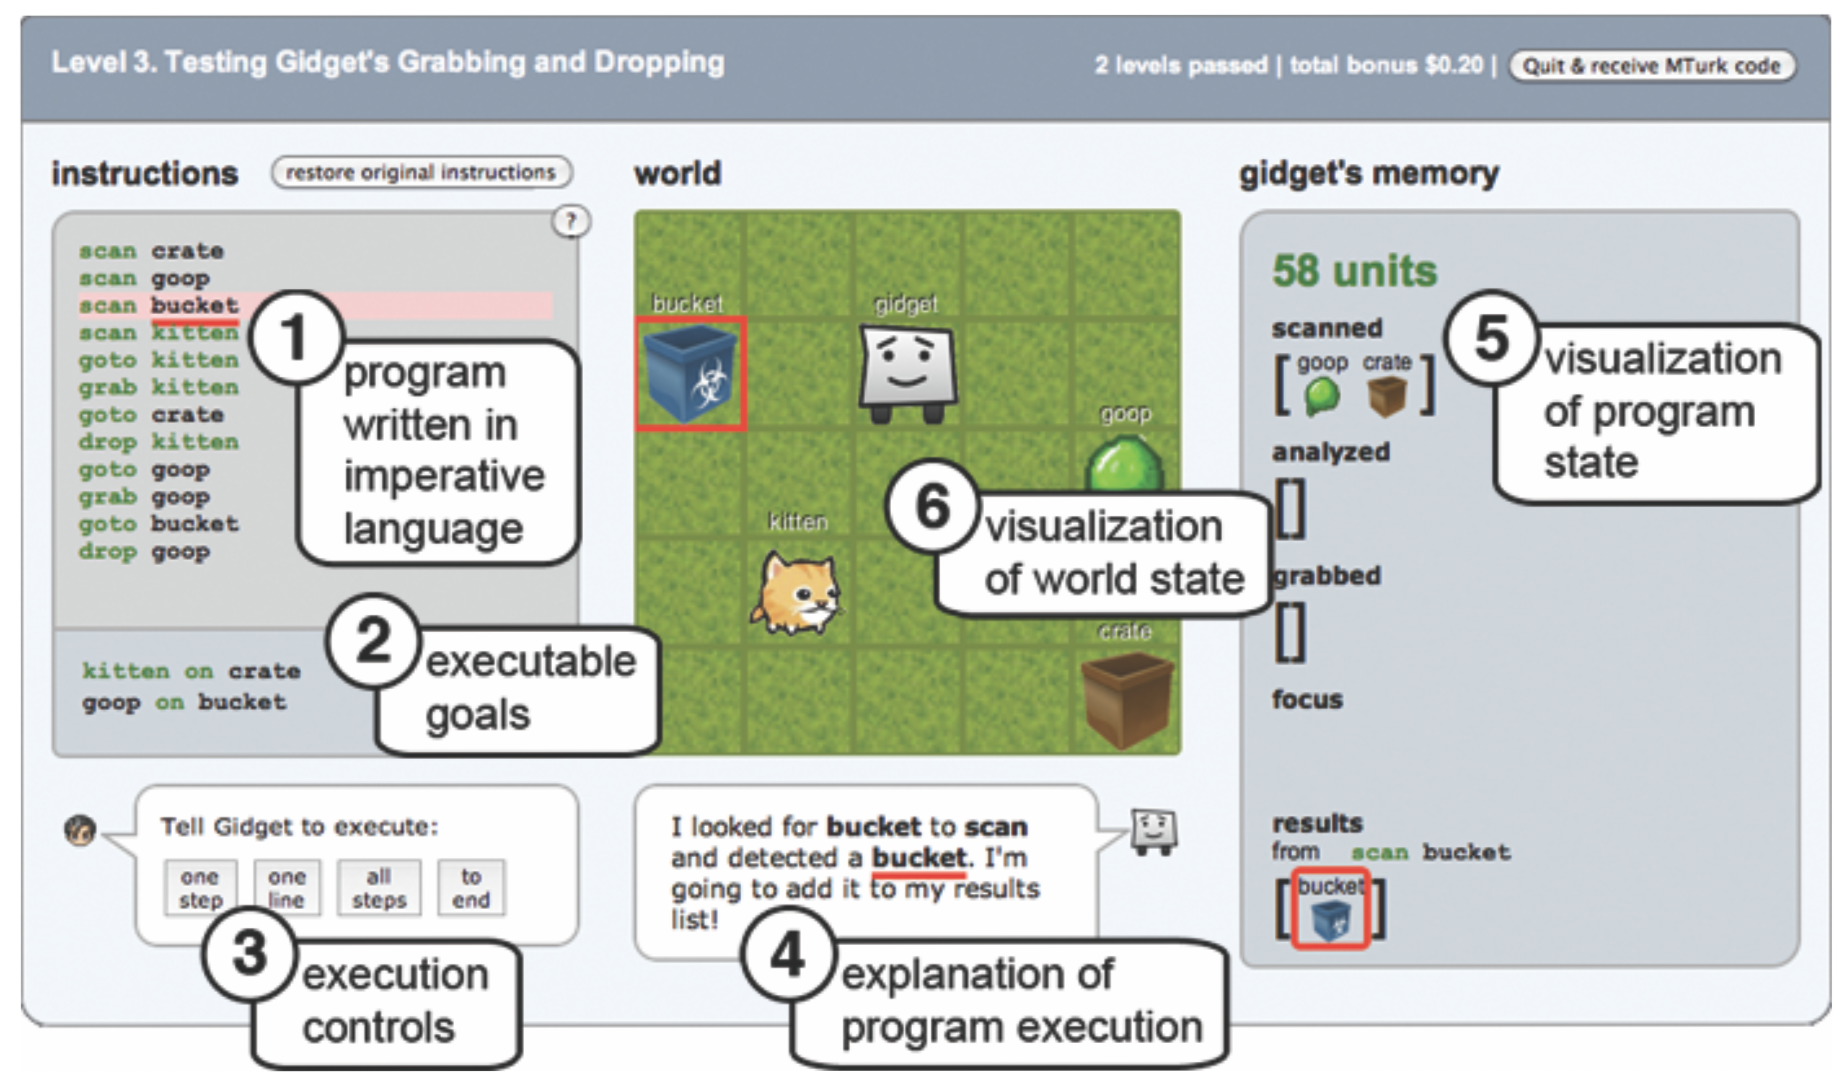
\includegraphics[width=1\textwidth]{Gidget-Example}
       \captionsetup{justification=centering}
\caption{A screenshot of the game Gidget {\citep{gidgetsite}}}
\label{fig:Gidget-Example}
\end{figure}


%\subsubsection*{Wu's Castle}



%\subsubsection{Gaming Platforms}

%Between 1997 and 2007, roughly 90\% of serious games were developed for personal computers, the other 10\% were made for a number of different home gaming consoles \citep{ratan2009}.








\section{Teaching Conditional and Iterative Control Structures}

%In 1985, the ACM education board teamed up with the IEEE Computer Society to produce a report of recommendations, for an introductory undergraduate computer science course \citep{tucker1991}. The latest report on computing curricula from ACM-IEEE was set out in 2013. This report covers the entire undergraduate computer science course, in which it describes a unit called 'Fundamental Programming Concepts', designed to be taught in the  first year of the course. This unit describes a set of programming topics that are "common to all programming paradigms" and that are "fundamental". One of these topics is 'Conditional and iterative control structures' \citep{acm}. 

In programming language design and implementation, 'control structure' refers to those constructs which determine the sequence of execution, of operations and statements within programs \citep{riccardi1981}. This definition is still relevant today \citep[see][]{wikiversity}. There are three types of control structures; sequential, conditional, and iterative \citep{leppanen2007}. A sequential structure is execution of a code line by line. A conditional construct is used to make decisions, for example, \textit{if} and \textit{if else} statements in JavaScript. An iterative construct is used for looping, for example, \textit{for} and \textit{while} loops in JavaScript.

These control structures are likely to be taught in larger introductory units, which cover a wide range of fundamental concepts \citep{acm}. For example, at the University of Bath, conditional and iterative structures are taught in semester 1 of year 1 of a computer science undergraduate degree \citep{bath}. 

%As iteration and conditional statements are very simple and quite fundamental, they are probably introduced and taught at the start of a course, for a brief period, and then used and built upon throughout the rest. Hence, I will look at methods for teaching introductory units as a whole.

%\subsection{Conditional and Iterative Control Structures}

%In programming language design and implementation, 'control structure' refers to those constructs which determine the sequence of execution, of operations and statements within programs \citep{riccardi1981}. This definition is still relevant today \citep[see][]{wikiversity}. There are three types of control structures; sequential, conditional, and iterative \citep{leppanen2007}. A sequential structure is execution of code, line by line. A conditional construct is used to make decisions, for example, \textit{if} and \textit{if else} statements in JavaScript. An iterative construct is used for looping, for example, \textit{for} and \textit{while} loops in JavaScript.

%These control structures are likely to be taught in larger introductory courses, which cover a wide range of fundamental concepts. For example, at the University of Bath, conditional and iterative structures are taught in semester 1 of year 1 of a computer science undergraduate degree \citep{bath}. As iteration and conditional statements are very simple and quite fundamental, they are probably introduced and taught at the start of a course, for a brief period. They are then most likely used and built on throughout the rest of the course. Hence, I will look at some methods for teaching introductory programming concepts.


\subsection{Methods}

At university, introductory programming units are conventionally structured courses based on lectures and practical laboratory work. Students learn about programming concepts through the programming language being taught \citep{Robins2003, acm}. \citeauthor{Robins2003} suggest that this approach is popular due to the programming knowledge that can be gained from the programming language, and the sheer volume and detail of language related features that can be covered.

Another method for learning iteration and conditional constructs, which is becoming increasingly popular is online resources. These resources include tutorial websites, such as Codeacademy and Khan Academy, which have accumulated millions of users, block-based programming environments such as Scratch and Alice, which provide creative visual environments, and educational games \citep{Lee2015}. 

In contrast, traditional methods of teaching centre on instructors who have control over class content and the learning process, whereas online resources, provide a learner-centred, self-paced learning environment \citep{Zhang2004}. \citet{Zhang2004} argue that e-learning could be used as an alternative to traditional classroom learning. Nevertheless, using e-learning to complement the learning process can make learning more effective and improve the learning experience \citep{Zhang2004, Concannon2005}

%Though a number of studies agree that serious games support learning, and used alongside other instructional methods, can make learning more effective and can improve the learning experience \citep{Pieter2013, Concannon2005, Granic2014}

%In comparison, traditional methods such as face-to-face or pencil-and-paper teaching \citep{Girard2013}, centers on instructors who have control over class content and the learning process, whereas, online learning, offers a learner-centered, self-paced learning environment. Online resources are also time and location flexible and provide unlimited access to learners \citep{Zhang2004}. 

%On the other hand, whilst there are many benefits to online learning, there are doubts over its effectiveness \citep{Zhang2004}. Some argue that online learning should not replace traditional forms of learning \citep{Zhang2004, Gunasekaran2002, agal2010}, instead it should be used to complement the learning process \citep{Zhang2004} and potentially improving the quality of the learners education \citep{Concannon2005}. Whilst other researchers highlight the great advantages of games over traditional methods \citep{Girard2013}.

%A meta-analysis conducted in 1992, looked at the empirical research on the instructional effectiveness of games to conventional classroom instruction.

\subsection{Issues}

%Teaching programming to novice programmers is regarded by some as a complex issue 

It is generally accepted that learning to program is a difficult task, and there are several problems associated with this \citep{Koulouri2014}. For leaners, the overhead of learning the syntax and semantics of a language at the same time, difficulties in combining new and previous knowledge, and developing their problem-solving skills, all add to the complexity of learning how to program \citep{Koulouri2014}.

There is also concern over the high drop out and failure rates of first and second year University students in computer science courses. This is potentially associated with considerable failure rates in introductory programming units \citep{Koulouri2014}. However, researchers have argued that there is little to no high-quality empirical data to support these claims \citep{bennedsen2007, watson2014}. In two different studies; \citet{bennedsen2007}, and \citet{watson2014}, both found that the failure rate of introductory units were 33\% and 33.3\%, from an average of 63 and 51 institutions respectively. Both studies argued that these rates were not "alarmingly high", but there is considerable potential for improvement \citep{watson2014}.

\citet{Koulouri2014} carried out 4-year study and found that certain implementations of introductory units, could improve student learning performance. One finding was that programming proficiency of novice programmers is dependent on the teaching approach of an introductory programming unit. Introductory programming units are also considered difficult \citep{watson2014}. In conclusion, choosing an approach that is engaging and motivating to teach fundamental programming concepts, is important.

%In a 4-year study with more than 750 participants, \citet{Koulouri2014} found that programming proficiency of novice programmers is dependent on the teaching approach of an introductory programming unit.

%\citet{Koulouri2014} suggested some changes to introductory units, that would improve the learning performance. 

%However it can be argued that since this study was released, computer science courses have changed drastically with respect to change in the discipline.
 


%Therefore careful consideration will be taken to reduce these problems, with efforts to; introducing programming concepts at a reasonable pace, and making the game fun and enjoyable to keep the user motivated. %Problems with teaching introductory programming to novices.

%have difficulty in tracing (mentally simulating the execution of the code before compiling), reading and understanding pieces of code. 


%Researchers have proposed guidelines as to what makes good intr3oductory programming units. For example, \citet{Stevenson2006} analysed assignments from textbooks and historical usage to look for students problems, and proposed a criteria as to what would make good programming assignments: (1) be based on real world problems, (2) allow students to generate realistic solution, (3) allow students to focus on current topic(s) within context of a larger problem, (4) be challenging, (5) be interesting, (6) make use of one or more APIs, (7) have multiple levels of challenge and achievement and finally (8) allow for some creativity and innovation.



\section{Educational Game Design}

%When researching the effects and effectiveness of digital games for learning, the importance of enjoyment for/in education needs to be taken into account. This means that when the effectiveness of a serious game is assessed, the question about its entertainment value should always be addressed \citep{Breuer2010}.

It is not sufficient to just assume that all forms of games are equally suitable for learning, and that simply presenting material in a game-like setting, will increase the quantity and quality of learning \citep{Breuer2010}. Designing educational games requires a focus that is different from general game design; otherwise, we may end up designing fun games with little or no learning value \citep{Barnes2007}.

\citet{Breuer2010} argue the ideal educational game combines entertainment and learning in a way that the players/learners do not experience the learning part as something external to the game. This idea of stealth learning should inform any approach to designing, using and evaluating educational games \citep{Breuer2010}. However, combining compelling and interactive design elements with specific curricular content that aims to retain learner's interest and attention, is a difficult task \citep{prensky2003}. 





%The design and production of video games involves aspects of cognitive psychology, computer science, environmental design, and storytelling, to name a few \citep{Koster2004}.

%\citeauthor{Driskell2002} describes a "tacit model that is inherent in most studies of instructional games". The model is as follows. Initially, we define a set of learning outcomes and objectives that we wish to achieve. We then design an instructional program which incorporates certain characteristics of games, that delivers the desired learning objectives. Subsequently, the program triggers a cycle that includes user judgments, user behaviours and system feedback. If the pairing of the instructional content with the appropriate game features is successful and effective, the cycle achieves recurring and self-motivated game play. Finally, this engagement in the game leads to the achievement of the learning outcomes \citep{Driskell2002}. This model is illustrated in Figure \ref{fig:Input_process_outcome_game_model}.

%\begin{figure}[H]
% \centering
%    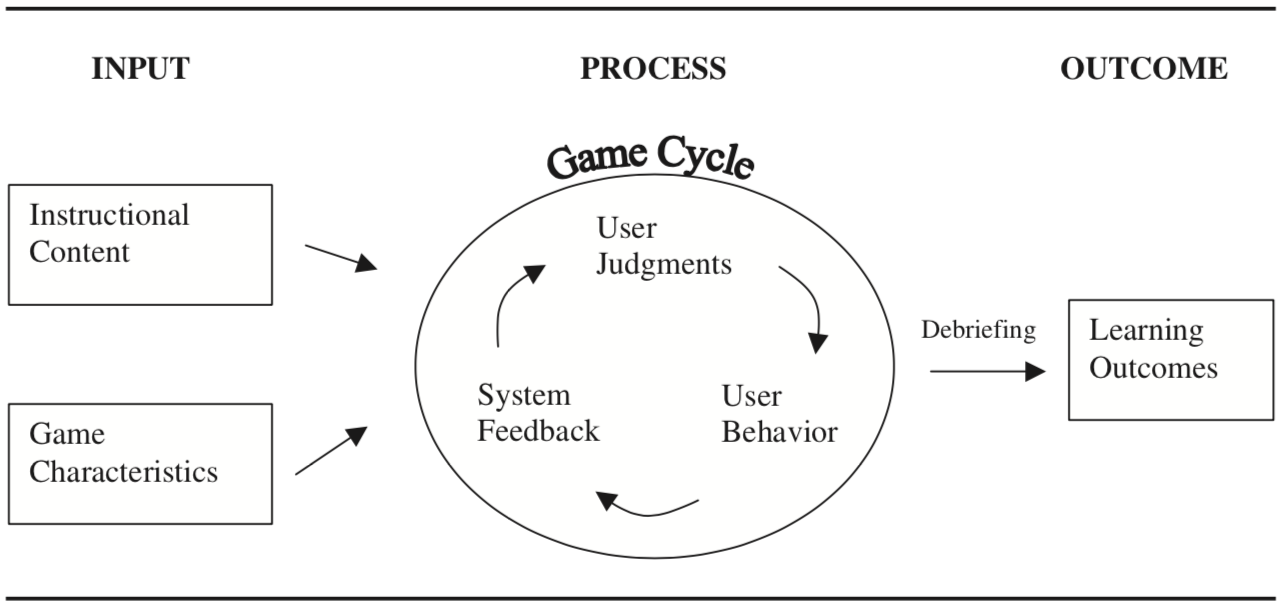
\includegraphics[width=1\textwidth]{Inputprocessoutcomegamemodel}
%      \captionsetup{justification=centering}
%\caption{Input-Process-Outcome Instructional Game Model  {\citep{Driskell2002}}}
%\label{fig:Input_process_outcome_game_model}
%\end{figure}


%Pleasure/fun and challenge have been found as some of the key reasons for people playing entertainment games \citep{Connolly2012}.

\subsection{Games and Learning}

Researchers have looked into the many factors that influence learning \citep{roungas2015}. Below are some of these factors that influence learning in a positive way, and how these are implemented in games. \citet{roungas2015} argue that these following factors are important and should be considered when designing serious games.

\subsubsection{Motivation}

Motivation is a key factor that drives learning. Without motivation, learning stops \citep{Gee2003}. A key factor of motivation is interest (Rousseau, 1762) (as cited in \citet{roungas2015}). Learning is effective when learners are interested in the material being taught and how it is presented. 

Games are natural sources of motivation. Games that bring about an optimal balance between challenge and frustration for players, is a very motivating state to be in \citep{Gee2003}. In his theory of flow, Csikszentmihaly describes that some leaners can become so focused in and absorbed by an activity that they lose track of time and completely ignore other tasks \citep{flow}. 

Researchers have looked into the intrinsic motivational properties of video games, that is, player motivation that arise due to factors within the players themselves. For example, pleasure and desire to develop a skill are forms of intrinsic motivations \citep{roungas2015}. \citet{Malone1987} investigated these properties of games, and presented a set of aspects of games that would make game-based learning more fun and engaging. The work by \citeauthor{Malone1987} is often referred to, but \citet{whitton2011} noted that Malone's work is not as valid today or as valid when considering adult engagement. With this, \citeauthor{whitton2011} described five aspects that lead to engagement specifically in games targeted for higher education: challenge, control, immersion, interest and purpose.

%Playing games is a fun and pleasurable activity \citep{Prensky2001}, and research has shown that fun and enjoyment are important part to the learning process, as learners can be more motivated and willing to learn \citep{Bisson1996, Cordova1996}. Games can also be very motivating and engaging \citep{Prensky2001}. They can leave players in an optimal balance of challenge and frustration, which can be a very motivating state for players \citep{Gee2003}.

\subsubsection{Repetition}

Repetition is considered crucial for learning, but some modern researchers do not consider it very important. However, it is deemed useful for learning skills such as programming \citep{roungas2015}, where it could be used for learning programming syntax and function names.

Repetition is very common in video games. It allows players to learn, memorise and potentially master some rules or controls of the game. Once players are familiar with these skills, the game then introduces a new problem, which requires players to integrate their old skills with new ones. These new problems are practised until a  problem requiring a different solution comes along. This cycle is repeated throughout the game \citep{Gee2003}.

However, repetition needs to be managed, as it could lead to boredom. To avoid this, \citet{roungas2015} suggest modifying the content of the task after each repetition. This can be achieved in games by slowly introducing new rules or controls that build upon previous game knowledge, or, by framing the task in different scenarios. \citet{roungas2015} also suggested managing how frequent the task is presented. A task repeated too often could lead to boredom, or a task repeated at very long time intervals, could reduce the learning benefits from repetition.


\subsubsection{Rewards}

The use of rewards and punishments in learning has various impacts. Firstly, rewards allow a learner to link learning with something pleasant. Secondly, rewards are form of extrinsic motivation, that is, learners are motivated by factors external to themselves. For example, achieving high grades, winning trophies or recognition by peers are all forms of extrinsic motivation \citep{roungas2015}. Thus attempting to seek such rewards may give learners motivation to continue their engagement with the activity. Finally, rewards were linked to increased learning performance in a study that used rewards in an educational game \citep{Filsecker2014}.

\citet{wang2011} goes as far as to say, rewards can foster intrinsic motivations, specifically, fun that arises from achieving rewards. An increase in intrinsic motivation in learners, has shown that learners are more deeply involved in activities and are more confident \citep{Cordova1996}. 

There are a variety of ways rewards can be expressed in video games, the following are some examples: score system, experience point system, item granting, resources, achievements, instant feedback, plot animations and unlocking mechanisms \citep{wang2011}. However, the relevancy and frequency of rewards needs to be managed, otherwise they can lead to diminishing returns; rewards should be suitable to the target audience, and like repetition, the frequency of rewarding is important. Rewarding too often can cause players to lose interest, or rewarding very little can lead players to lose motivation to play \citep{roungas2015}.


\subsection{Game Elements} %Important characteristics of games

Games have several characteristics. \citet{roungas2015} argue the following characteristics are important for serious game design. These characteristics are aimed at keeping games engaging, exciting and educational.

\begin{enumerate}
	\item \textbf{Rules}. Rules are essential to a game. They describe how the game works and limit the players' actions \citep{roungas2015}. Whilst surveying players of introductory programming games, \citet{Barnes2007} gathered that rules should be provided and accessible throughout the game. This would allow players to refer back to the rules during the game in case they needed reminding or help.

	\item \textbf{Goals}. Goals allow players to judge their performance. They also act as a motivation for players \citep{roungas2015}. \citep{Barnes2007} found that goals should also be provided and accessible throughout the game. They must be clearly tied to in-game feedback, such as avatar health or score, that either motivates or penalises players \citep{Barnes2007}.
	
	\item \textbf{Challenge}. Challenge leads to engagement, if, tasks are optimally balanced between challenge and skill \citep{whitton2011, flow}. Challenges need to be carefully designed in order to not be too boring or too difficult \citep{roungas2015}.
	
	\item \textbf{Feedback}. Feedback allows players to assess their performance \citep{roungas2015}. It leads players towards correct answers if their assumptions are wrong, and thus creates learning opportunities. However in programming, feedback in the form of errors can be quite discouraging to novice programmers \citep{lee2011}. Thus care should be taken when designing feedback in a beginner programming game. Feedback should be presented clearly and on time \citep{roungas2015}.
\end{enumerate}

%EFM: A Model for Educational Game Design

%Game object model version II: a theoretical framework for educational game development (318)

%Game, motivation, and effective learning: An integrated model for educational game design (230)

%Serious Games: A New Paradigm for Education?







%In 1980, Thomas W. Malone had begun researching the natural motivational properties of video games. With this work Malone created a set of heuristics based on motivational principles of games to create fun instructional game designs \citep{Malone1987}.  In 1996, Lloyd Rieber Z

%Rieber, and others [100] argued that his fantasy element leads to engagement with the learning content. Here then, in the work of Rieber we have a logical extension of the approach of Malone ? that is the segmenting of ?games? into a set of heuristics that can be used to form Serious Games design.

%This work to unpack, stratify demarcate, or otherwise categorize games into a set of heuristics or design principles to be applied to educational games was a significant focus for researchers at the time [101]. Moreover, when reviewing the modern trends in Serious Games research, it is apparent that this trend has continued ? though the models are now more formalised [38, 102?104]






%\subsection{Game Genre}

%Simulation games are one of the most common game genres in serious games, possibly because their use in education is already established \citep{Connolly2012}. Simulation games have the ability to represent real-life situations \citep{Braghirolli2016}. 

%https://www.researchgate.net/publication/272166351_A_taxonomy_of_educational_games

%To encourage the use of games in learning beyond simulations and puzzles, it is essential to develop a better understanding of the tasks, activities, skills and operations that different kinds of game can offer and examine how these might match desired learning outcomes \citep{Connolly2012}.





%\subsection{Game Elements}

%(CHANGE IT UP) \citeauthor{Barnes2007} ran a project that made University Students create games that would teach basic programming. They carried out evaluations to test participant learning from the game, and made some interesting observations as follows: Clear instructions and game goals must be provided and accessible throughout the game, Learning goals must be clearly tied to in-game feedback that motivates the player (through, e.g. experience points, health), and penalizes guessing, Humor can be a motivation for in-game interaction \citep{Barnes2007}.

%rewards remain controversial in education due to their possible negative side effects on individuals motivation, Despite the controversy concerning the use of external rewards in education (Cameron, Pierce, Banko, \& Gear, 2005). badges in the context of a technology-based innovation in an elementary school can enhance learning without undermining motivation \citep{Filsecker2014}.

\afterpage{\blankpage}





\chapter{Requirements Specification}

%This chapter should identify the process of requirements capture and analysis that was adopted (explaining why a particular technique or method was adopted rather than competing techniques, if necessary). The section should identify and discuss key requirements, and focus particularly upon areas of particular challenge, difficulty or conflict. An appropriate scoping of the desired system is a key part of any project, reflecting an appropriate understanding of the resource limitations that impinge on the project. The chapter should be careful to identify areas of the process of requirement analysis and specification which were particularly ?successful? or demonstrate good practice, and be appropriately self-critical of areas where difficult compromises have had to be made.

The literature review highlights several key areas of study that were used to inform the requirements specification. The following parts of the literature review will be considered; benefits of educational games; issues of teaching iterative and conditional control structures; the elements from the example of educational games that had a positive impact, and finally educational game design.

The requirements are split into functional and non-functional sections, and each requirement is given an importance rating of: high, medium or low, which refer to being essential, conditional or optional for the system respectively. 

The aim of the current study is to develop an educational game to teach iterative and conditional control structures. This will be achieved through the following requirements:
%which part of lit review will requirements spec consider. (pedagogical requirements and gamification requirements.)


%The pedagogical requirements were mostly informed by research done in section 2.2, which... these requirements address decisions such as what are the learning objectives of the game, and how much detail should it go into on these topics





\section{Non-Functional Requirements}

\begin{enumerate}[label=3.1.\arabic*]

  \item \textbf{Game must be easily accessible from home, work or school.} A key benefit of e-learning over traditional forms is being able to access learning material at any time, given a device with an internet connection and a browser \citep{Girard2013}. \newline Priority: High

  \item \textbf{Game must improve player's knowledge on iterative and conditional control structures.} A key requirement of a serious game is to educate the player. \newline Priority: High
  
  \item \textbf{Game must not assume player has any existing programming knowledge.} Iterative and conditional constructs are fundamental programming concepts, and the target audience is assumed to have little to no programming knowledge. \newline Priority: High
  
  \item \textbf{Game should have a reasonable difficulty curve.} Players should be able to learn the basic game controls early on in the game. Game should then get progressively harder, keeping the player challenged and engaged. \newline Priority: Medium
  
  \item \textbf{Game should be fun and enjoyable to play.} Entertainment is not the primary purpose of the game. However experiencing fun and enjoyment whilst playing helps improve players' learning performance \citep{giannakos2013}. \newline Priority: Medium
  
  \item \textbf{Player should be motivated throughout the game.} Motivation is a key aspect that drives learning \citep{Gee2003}. \newline Priority: Medium
  
  \item \textbf{Player should feel challenged.} Challenge is described as one of the aspects that leads to player engagement \citep{whitton2011}. \newline Priority: Medium
  
  \item \textbf{Game may foster player motivation to learn more complex programming.} Player motivation, specifically student motivation in computer science courses is a concern, and can be improved. \newline Priority: Low
  
\end{enumerate}


\section{Functional Requirements}

\begin{enumerate}[label=3.2.\arabic*]

  \item \textbf{Game rules and goals must be accessible throughout the game.} Players must be able to refer back to the rules and goals throughout the game. \newline Priority: High

  \item \textbf{Game must at least introduce \textit{if} statements and \textit{for} loops.} These constructs can be considered very basic and essential iterative and conditional control structures. \newline Priority: High
  
  \item \textbf{Game must define in-game functions to be used with \textit{if} statements and \textit{for} loops.} This will allow to merge the educational goals of the game with its entertainment aspect. \newline Priority: High
  
  \item \textbf{Game must have levels with clear defined goals, that require increasingly difficult solutions.} Clear accessible goals will tell the player what to do each level. Concepts can be introduced at a reasonable pace, that work to limit player overwhelm. \newline Priority: High
  
  \item \textbf{Game must give players some control over choice of action.} Learner control is an aspect that is not widely present in most traditional forms of teaching, and control is described to lead to greater engagement \citep{whitton2011}. \newline Priority: High

  \item \textbf{Game must give feedback to player solutions.} Feedback is important as it allows players to assess their performance and deal with any mistakes. \newline Priority: High
  
  \item \textbf{Game must use some form of in-game rewards and punishments, such as score points and hit points.} The use of game rewards and punishments foster extrinsic motivations, encouraging player engagement \citep{roungas2015}. \newline Priority: High
  
  \item \textbf{Game must have a general help section.} Players could use this as a reference point throughout the game. \newline Priority: High
  
  \item \textbf{Game should give feedback in a personal and constructive way.} Impersonal feedback on programming errors can reduce player motivation, whilst constructive feedback can improve motivation. \newline Priority: Medium

  \item \textbf{Game should be web-based, and playable in three most popular web browsers.} These are Chrome, Safari and Firefox \citep{statistabrowser}. Allows the game to be widely accessible.  \newline Priority: Medium
  
  \item \textbf{Game should have a tutorial to introduce the game rules, goals and game mechanics.} The tutorial will be able immediately introduce the core concept of the game including the educational aims. \newline Priority: Medium
  
  \item \textbf{Game may provide tips to the player about individual level.}  In case player is ever stuck on a level, tips would help the player progress. \newline Priority: Low 
  
  \item \textbf{Game may save players progress.} Saving game state would allow players to exit the game for any reason, and return any time they wish. \newline Priority: Low
  
  \item \textbf{Game may educate the player about functions and parameters.}  In-game functions of the form of actual programming functions, may familiarise players about the use of functions and passing in parameters. \newline Priority: Low
  
\end{enumerate}


\afterpage{\blankpage}






\chapter{Design}

% The design chapter will typically address the problem of method choice, but should not simply regurgitate the well-known details of myriad competing design methods. The chapter should then introduce the overall architecture of the design (the high-level design) so that the reader can gain an understanding of the approach being adopted. The chapter should not be allowed to become a catalogue of key classes or design components. Instead, it should select key parts of the design which are particularly important, illustrate the selection of particular approaches from a range of possible design decisions, or show the application of particular design patterns for the solution of identified problems. Of particular importance are areas of the design which resolve key viewpoint conflicts that were identified in requirements capture and analysis.

%If the user interface specification and design is an important part of the project, then it may be appropriate to dedicate a separate chapter to this component of the system. It is common for project students to spend considerable time rehearsing principles of user interface design that are readily accessible from key texts. Whilst it is important that these principles are used and applied, extensive regurgitation of this material is often unnecessary and simple reference can be made to the appropriate sources. If, however, the project is investigating new approaches to user interface development, then a more in-depth consideration of the principles of user interface design may be appropriate in the literature and technology survey.


%Mechanics describes the particular components of the game, at the level of data representation and algorithms.

%Dynamics describes the run-time behaviour of the mechanics acting on player inputs and each others' outputs over time.

%Aesthetics describes the desirable emotional responses evoked in the player, when she interacts with the game system.

Since the start of the project, the idea for the genre of the game was a 2D maze adventure. Researchers have argued which genres of games are best suited for educational purposes \citep{moreno2008}, however most of the discussion on educational game design does not revolve around the game genre, but instead on which game elements, pedagogical concepts and player feelings aroused by the game are most important. These aspects were discussed in the literature review and were used to inform and influence the requirements specification. This chapter aims to indicate how the problem, as specified within the requirements, is analysed to create a potential solution.

\section{Core Idea}

The core idea of the game is a character stranded in a dungeon, and the user must write pieces of code to control the character and help him escape. To do this, the user is given a set of pre-defined functions to use to control their character. These pre-defined functions will simply be referred to as 'functions' throughout this study. Throughout the game, users are slowly introduced to \textit{if} statements and \textit{for} loops, which they then must use with the functions to create pieces of code. The aim is for users to initially create simple pieces of code, then move onto creating more complex structured and efficient code as they progress.

To help discuss the design, the goals of the game are split into two. The first goal, and also the aim of this study, is to educate users on certain iterative and conditional control structures. These will be referred to as the educational goals. The second goal is to help the in-game character escape. This will be referred to as the game goal.

\section{Web-based}

%Intro + Reason
%HTML and JavaScript

A web-based design was adopted to develop the game. A web game has several advantages over other forms of video games. Namely, these are:

%Compatibility is another huge advantage HTML5 has. HTML is the lowest common denominator for all web based devices. By using HTML5 you can target a wider array of devices and gadgets without having to specifically port your game to each different platform. Another often forgotten advantage is ease of use. For the technically savvy, downloading, installing, and updating plug-ins is only a minor hassle. However, for less technically savvy users this can be quite a hurdle and just may turn away users altogether.

\begin{itemize}

	\item Accessible on most web browsers without having to create different versions of the game for each browser. This is cost-effective and reduces hassle for users.
	\item Accessible through a number of different web-based devices, without having to create different versions of the game or install the game onto each different device. This allows the game to be accessible in more places. 
	\item Ease of accessibility, given that computers with an internet connection are ubiquitous. Only requires a browser to play.
	\item Requires no additional download, installation or update to plug-ins. Reduces the complexity needed for users to access the game.
	\item Easy to update web applications once they are deployed. Requires no update from user to get the latest version of the game, apart from perhaps updating their web browser to the latest version.
	\item Can achieve greater levels of interoperability compared to desktop environments \citep{roungas2015}.
	
\end{itemize}


\section{Game Mechanics} %What I want to achieve (player moves through dungeon through use of programming)

%Functionality of game.
%The following subsections will discuss the elements of the game that the user directly interacts with, or interactions that occur through users action.



Game mechanics can be defined as the methods invoked by agents for interacting with the game world \citep{sicart2008}. In the context of this game, the agents are the players and the methods are those elements of the game, that the user interacts with either directly or through their actions, that effect the game state. The following subsections will discuss these elements in more detail and the justification for their adoption.

\subsection{Functions}

Commonly when using \textit{if} and \textit{for} constructs, statements are defined within the construct to be executed. For this game, functions that help the in-game character, were decided to be used as such statements. Furthermore, the use of functions to control in-game characters had a positive impact on the engagement of players in the educational game Prog\&Play.

Four functions were designed, and these can be split into two types. One type to control the characters actions: walk or shoot. The other type to be used as conditions in \textit{if} and \textit{else if} statements, which would return true or false based on facts about the game state: if a wall is nearby, or, if an enemy is nearby.

Throughout the game players would have to use these functions within \textit{if} statements and \textit{for} loops to help achieve the game goal, in turn helping them achieve the educational goals. Thus these functions can be seen as the bridge between the entertainment aspect of the game and the educational aims. 

However as discussed in the literature review, care needs to be taken when trying to introduce programming to novice programmers. They can often struggle with the complexity of the syntax and semantics of the programming language. To tackle this issue, the aim is to dissipate the introduction of these functions and constructs throughout the game, which will be discussed in more detail in the level design section. This is also why only four functions were designed that take one of four parameters: left, right, up or down. Helping reduce the complexity of the game.

\subsection{Scoring}

Score is an essential aspect in many video games. It provides players feedback based on their performance, and create opportunities for them to want to improve.

As control was an important aspect for engagement, players will be able to control the solution they came up with for a level. Thus implementing a scoring system that would judge the quality of a code would be a very complex task. Instead, a scoring system that judges players based on the time taken to complete a level was decided.

The design of the scoring system would be to give players a fixed score at the start of the game, which would immediately begin to decrease. Upon completion of a level, the same fixed amount would be added to the players' score, and would then continue to decrease from this new amount. This would carry on until the player completed the game and was presented with their final score.

This style of scoring system challenges players to want to come up with solutions quickly and thus engaging players. However a drawback may be that players get frustrated if they feel forced to come up with a solution quickly. To tackle this, the fixed amount a score would increase by, would be a large number, and the score would decrease very gradually. Thus potentially decreasing players' temptation to rush as they are likely to end up with a high score. Players can feel joy about achieving a high score, and still feel engaged and challenged.

\subsection{Hit points}

%Why it is necessary
%Design 
%Impacts
%Issues
%Any other hit points systems?


\section{User Interface} %How it will look ()

\subsection{Dungeon}

\subsection{Console}


\section{Level Design} %How game progresses (what is learnt each step of the way)

\subsection{Tutorial}




\afterpage{\blankpage}


\chapter{Implementation}

%This chapter will follow the same approach as the Design chapter, presenting an overview of the software architecture and a high-level discussion of the implementation process. It will reflect on appropriate implementation approaches, algorithm choices and language choice, using the more detailed discussion provided within the literature and technology survey to justify decisions taken. It will include discussion of any ancillary techniques used to ease implementation (such as the use of source code control systems and associated release plans). The discussion should not descend to become a simple catalogue of classes or methods, but should select non-trivial components, interesting implementation techniques, or important algorithm choices to discuss. It is important to take time to decide which design and implementation issues warrant discussion and which do not.

\section{Technologies Used}

\section{System Architecture}

\section{Functions}

\subsubsection*{Player.move()}

\subsubsection*{Player.shoot()}

\subsubsection*{wallPosition()}

\subsubsection*{enemyPosition()}

\afterpage{\blankpage}




\chapter{Testing}

\section{System Testing}

\section{User Testing}
\subsection{Observed Playthroughs} %Think aloud protocol, initial testing
\subsection{Questionnaires}

Useful literature:
Purposeful by design?: a serious game design assessment framework

\afterpage{\blankpage}




\chapter{Results}

\section{System Improvement}

\section{Usability}

\section{Learning}

\section{Engagement}

\afterpage{\blankpage}




\chapter{Discussion}
\afterpage{\blankpage}



\chapter{Future Work}

Here, it is important that not only the final outcomes are assessed, but also that the learning and training process itself is monitored continuously without impairing the playing/learning experiences (e.g. via psycho physiological measurements or automated logs/recordings of player behaviour). This is especially beneficial as it can inform new ways to make learning games more adaptive so that they can always offer help or additional information when the players need it (e.g. when they get stuck at a certain point of a game) \citep{Breuer2010}.

\afterpage{\blankpage}


\bibliography{litreview}
\addcontentsline{toc}{chapter}{Bibliography}


\appendix
\addtocontents{toc}{\protect\setcounter{tocdepth}{-1}}
\addtocontents{toc}{\protect\setcounter{tocdepth}{0}}
\appendixpage

\renewcommand\chaptername{Appendix}
%\chapter{Technical Specification and GA of the Skyseeker}\label{app:techspec}

\newpage
\chapter{Uncertainty Analysis} \label{app:errors}

\chapter{Screenshots} \label{app:screenshots}

\chapter{Ethics Checklist} \label{app:ethicschecklist}

\end{document}  